\documentclass[12pt]{report}
\usepackage{%
	amsfonts,%
	amsmath,%	
	amssymb,%
	amsthm,%
	algorithm,%
	babel,%
	bbm,%
	etex,%
	%biblatex,%
	caption,%
	centernot,%
	color,%
	dsfont,%
	enumerate,%
	epsfig,%
	epstopdf,%
	geometry,%
	graphicx,%
	hyperref,%
	latexsym,%
	mathtools,%
	multicol,%
	pgf,%
	pgfplots,%
	pgfplotstable,%
	pgfpages,%
	proof,%
	psfrag,%
	subfigure,%	
	tikz,%
	ulem,%
	url%
}	
\usepackage[noend]{algpseudocode}
\usepackage[mathscr]{eucal}
\usepgflibrary{shapes}
\usetikzlibrary{%
  	arrows,%
	backgrounds,%
	chains,%
	decorations.pathmorphing,% /pgf/decoration/random steps | erste Graphik
	decorations.text,%
	matrix,%
  	positioning,% wg. " of "
  	fit,%
	patterns,%
  	petri,%
	plotmarks,%
  	scopes,%
	shadows,%
  	shapes.misc,% wg. rounded rectangle
  	shapes.arrows,%
	shapes.callouts,%
  	shapes%
}

\theoremstyle{plain}
\newtheorem{thm}{Theorem}[section]
\newtheorem{lem}[thm]{Lemma}
\newtheorem{prop}[thm]{Proposition}
\newtheorem{cor}[thm]{Corollary}

\theoremstyle{definition}
\newtheorem{defn}[thm]{Definition}
\newtheorem{conj}[thm]{Conjecture}
\newtheorem{exmp}[thm]{Example}
\newtheorem{assum}[thm]{Assumptions}
\newtheorem{axiom}[thm]{Axiom}

\theoremstyle{remark}
\newtheorem{rem}{Remark}
\newtheorem{note}{Note}
\newtheorem{fact}{Fact}

\newcommand{\norm}[1]{\left\lVert#1\right\rVert}
\newcommand{\indep}{\!\perp\!\!\!\perp}
\DeclarePairedDelimiter\abs{\lvert}{\rvert}%
\newcommand\numberthis{\addtocounter{equation}{1}\tag{\theequation}}
\newcommand{\tr}{\operatorname{tr}}
\newcommand{\R}{\mathbb{R}}
\newcommand{\N}{\mathbb{N}}
\newcommand{\E}{\mathbb{E}}
\newcommand{\Z}{\mathbb{Z}}
\newcommand{\B}{\mathscr{B}}
\newcommand{\C}{\mathcal{C}}
\newcommand{\T}{\mathscr{T}}
\newcommand{\F}{\mathcal{F}}
\newcommand{\G}{\mathcal{G}}
%\newcommand{\ba}{\begin{align*}}
%\newcommand{\ea}{\end{align*}}
\DeclareMathOperator*{\argmax}{arg\,max}
\renewcommand{\qedsymbol}{$\blacksquare$}
\makeatletter
\def\BState{\State\hskip-\ALG@thistlm}
\makeatother

\makeatletter
\def\th@plain{%
  \thm@notefont{}% same as heading font
  \itshape % body font
}
\def\th@definition{%
  \thm@notefont{}% same as heading font
  \normalfont % body font
}
\makeatother
\date{}
\usepackage{scribe_e1244}
\usepackage{times}
\begin{document}
\lecturer{Aditya Gopalan}		% optional, put lecturer's name here
\scribe{Firoz shah , Vaidya Dhavalkumar B}					% required, put your name here
\lecturenumber{2}						% required, must be a number
\lecturedate{January 5}					% required, omit year
\maketitle

\section{Recap}
Setup for statistical Hypothesis testing considering Binary Hypothesis testing with Bayesian assumption.\\
 {$\Gamma$: Observation Space. }\\
{$\delta$: Decision rule/Hypothesis test.}\\ 
{$\delta: \Gamma \to \{0, 1\}$}\\
{$\mathbb{P}_0$ and $\mathbb{P}_1$  are pdf associated with $H_0$ and $H_1$ respectively.}\\

\begin{figure}[h]
\centering
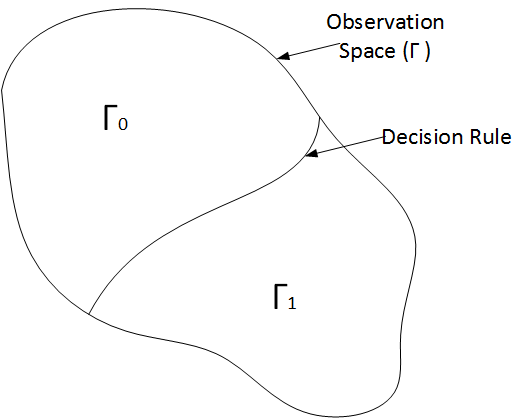
\includegraphics[scale=0.5]{Figures/ObservationSpace}
\caption{Depiction of observation space and decision rule.}
\label{fig:obsspace}
\end{figure}

\begin{itemize}
\item {\bf \em Costs}: $C_{i,j}$: Cost of deciding hypothesis $H_i$ when hypothesis $H_j$ was actually true.
\item {\bf \em Conditional Risk}: To evaluate the performance of decision rule 
 $R_j$:Expected cost of $\delta$ when hypothesis j is true.
\begin{align*}
R_j(\delta) &\bydef \mathbb{E}_j\left[ C_{j0}\indic{Y \in \Gamma_0} + C_{j1}\indic{Y \in \Gamma_1} \right] \\
&= C_{j0} \, \mathbbm{P}_j[\Gamma_0] + C_{j1} \, \mathbbm{P}_j[\Gamma_1].
\end{align*}
\item {\bf \em Bayesian assumption}: Hypothesis  $H_0$ and $H_1$ occur with prior probablities $\pi_0$ and $\pi_1$ respectively.\\
$\pi_0 + \pi_1 = 1$ , $\pi_0 \ge 0$, $\pi_1 \ge 0$
\item {\bf \em Bayes risk of $\delta$}: Rules that minimize r($\delta$)
\begin{align}
r(\delta) &\bydef \pi_0 R_0(\delta) + \pi_1 R_1(\delta) \\
\nonumber
\end{align}
A Bayes rule $\delta_B$ has the following form $\forall y \in gamma$.\\
\[ \delta_B(y) = \left\{ 
\begin{array}{cc}
1, &  \text{if }\sum_{j=0}^1 \pi_j \left( C_{1j} - C_{0j} \right) p_j (y) \leq 0 \\
0, &  \text{if }\sum_{j=0}^1 \pi_j \left( C_{1j} - C_{0j} \right) p_j (y) > 0. \\
\end{array}
 \right. \]
\section{Notes}
\begin{note}
Bayes rules are likelihood ratio tests(LRT's)
\end{note}
For the Bayes rule, \\
\begin{eqnarray}
\centering
\nonumber
\Gamma_1 &\bydef& \{y \in \Gamma: \delta(y) = 1\}.\\
%
\nonumber
&=&\{y \in \Gamma: \pi_0  \mathbbm{P}_0(y) \left(C_{10}-C_{00} \right) \leq \pi_1  \mathbbm{P}_1(y) \left(C_{01}-C_{11} \right)\}\\
\nonumber
\text{Assume}C_{01} \ge C_{11}\\
\nonumber
&=&\{y \in \Gamma: \frac{p_1(y)}{p_0(y)} \geq  \frac{\pi_0 (C_{10}-C_{00} )}{\pi_1 (C_{01}-C_{11} )}\}\\
\nonumber
\end{eqnarray}
$p_1(y)$ :Probability that y is produced by hypothesis 1\\
$p_0(y)$ :Probability that y is produced by hypothesis 0\\
\begin{align*}
\noindent
L(y) \bydef \frac{p_1(y)}{p_0(y)} = \text{"Likelihood ratio of y} \in \Gamma \\
\noindent
\Gamma_1 = {y \in \Gamma : L(y) \geq \tau }\\
\end{align*}
\begin{align*}
\noindent
\text{Where      }  
 \tau \bydef \frac{\pi_0 (C_{10}-C_{00})}{\pi_1 (C_{01}-C_{11})} (Threshold)\\
\noindent
\text {Hence Bayes rules are likelihood ratio tests (LRT's)} 
\end{align*}
\begin{note}
The Bayes' rule under Uniform Cost Structure
\end{note}
A commonly used cost assignment is the uniform cost structure. In uniform cost structure, the cost while making wrong decision (meaning choosing wrong hypothesis) is given as, 
\begin{align*}
 C_{ij} =  \indic{i \ne j}  \\
\end{align*}
 and no cost for choosing right hypothesis.

\begin{figure}[h]
\centering
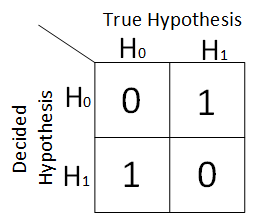
\includegraphics[scale=0.7]{Figures/UniformCostTable}
\caption{Uniform Cost Table for Binary Hypothesis Testing.}
\label{fig:uniformcost}
\end{figure}


The Bayes rule $\delta_B$, here is simplified as (under uniform cost structure),
\begin{align*}
\Gamma_1 =\{y \in \Gamma : L(y) \geq \frac {\pi_0}{\pi_1}\}
\end{align*}
The RHS of the inequality denotes the "Prior Probabilities"\\
so the threshold $(\tau)$ is ratio of prior probabilities.\\
and the Bayes' risk can be calculated as,
\begin{eqnarray}
\nonumber
r(\delta)&= \pi_0 R_0 + \pi_1 R_1 \\
\nonumber
\end{eqnarray}
Here,
\begin{eqnarray}
 R_0 &= C_{00}  \mathbbm{P}_0[\Gamma_0]+C_{10}  \mathbbm{P}_0[\Gamma_1]\\
\nonumber
\end{eqnarray}
But we pay cost only when the wrong hypothesis is chosen, 
\begin{eqnarray}
\nonumber
C_{00}&=0,C_{10}=1\\
\nonumber
\end{eqnarray}
Hence, 
\begin{eqnarray}
\nonumber
R_0&=  \mathbbm{P}_0[\Gamma_1]\\
\nonumber
\end{eqnarray}
Similarly,
\begin{eqnarray}
\nonumber
R_1&=  \mathbbm{P}_1[\Gamma_0]\\
\nonumber
\end{eqnarray}
Therefore,
\begin{eqnarray}
\nonumber
r(\delta)&=& \pi_0  \mathbbm{P}_0[\Gamma_1]+\pi_1  \mathbbm{P}_1[\Gamma_0]\\
&=&\mathbbm{P}[\{H_0 \text{ is true , }  \delta_B(y) = 1\}  \cup \{H_1  \text{ is true , } \delta_B(y) = 0\}]
\nonumber
\end{eqnarray}


\noindent
We define an ERROR event $E$ as follows:
\begin{align*}
E = \{H_0 \text{ is true , }  \delta_B(y) = 1\}  \cup \{H_1  \text{ is true , } \delta_B(y) = 0\}
\end{align*}
then $r(\delta) = P[E]$\\
Hence, for uniform cost structure the Bayes' rules are minimum probability of error rules.
\begin{note}
Connection with Bayes' formula (used to calulate the conditional probability)\\
Given an observation $y\in\Gamma$, the posterior probabilites of $\mathcal{H}_j$ for $j\in\{0,1\}$
\begin{align} 
\pi_j(y) = \Pr\{ \mathcal{H}_j \text{ is true } | Y = y \} &= \frac{\Pr\{ Y=y | \mathcal{H}_j \text{is true} \}\Pr\{ \mathcal{H}_j \text{is true}\}}{\Pr\{Y=y\}}\\
&=\frac{\Pr\{ Y=y | \mathcal{H}_j \text{is true} \}\Pr\{ \mathcal{H}_j \text{is true}\}}{\pi_0P_0(y) + \pi_1P_1(y)}\\
&=\frac{P_j(y)\pi_j}{\pi_0P_0(y) + \pi_1P_1(y)}
\end{align}
Let, 
\begin{align*} 
P(y) =\pi_0P_0(y) + \pi_1P_1(y)
\end{align*}
A Bayes' rule under general cost structure $\delta_B$ is,
\begin{align*} 
\Gamma_1 &= \{ y\in\Gamma : \sum_{j}\pi_j(C_{1j}-C_{0j})P_j(y) \leq 0\}\\
&=\{ y\in\Gamma : \sum_{j}\pi_j C_{1j} P_j(y) \leq \sum_{j}\pi_j C_{0j} P_j(y) \}\\
&=\{ y\in\Gamma : \sum_{j}\frac{\pi_j C_{1j} P_j(y)}{P(y)}  \leq  \sum_{j}\frac{\pi_j C_{0j} P_j(y)}{P(y)}\}\hspace{10 mm}\text{Both side is divided by P(y)$>$0}\\
&=\{ y\in\Gamma : \sum_{j}\pi_j(y) C_{1j}  \leq \sum_{j}\pi_j(y) C_{0j}\}
\end{align*}
The terms $\sum_{j}\pi_j(y) C_{1j}$ and $\sum_{j}\pi_j(y) C_{0j}$ has special meaning,\\
Expanding the first term,\\
\begin{equation}
\nonumber
\sum_{j}\pi_j(y) C_{1j} = C_{10} \pi_0(y) + C_{11} \pi_1(y)
\end{equation}
is the average cost incurred by choosing hypothesis $\mathcal{H}_1$ given that $Y$ equal $y$. This quantity is called the posterior cost of choosing $\mathcal{H}_1$ when the observation is $y$, and thus Bayes' rule makes its decision by choosing the hypothesis that yields the minium posterior cost.\\
LHS:\hspace{10 mm}$\sum_{j}\pi_j(y) C_{1j} = $ Bayes' risk of a rule that always outputs 1, under prior ($\pi_0(y),\pi_1(y)$)\\
RHS:\hspace{10 mm}$\sum_{j}\pi_j(y) C_{0j} = $ Bayes' risk of a rule that always outputs 0, under prior ($\pi_0(y),\pi_1(y)$)
\end{note}
Now we will look at two examples for Bayesian Hypothesis Testing.

\begin{exmp}[The Binary Channel]
The binary channal is very commonly used in communication. It accepts bit  $0$ or $1$ and outputs bit $0$ or $1$. It acts like a function which accepts one bit input and produces one bit output depending upon the characteristics of the channel. The noise present in the channel may flip the bit at the output. The decision rule at the receiver needs to decide what is the actual bit transmitted from the transmitter side based on the observation made at the receiver side
\par Let $Y$ be the observation at the output of the receiver, which can be either $0$ or $1$. Let the bit flipping probability (due to noise present in the channel or due to some other imperfaction present in the channel) be $\lambda_0$ when bit $0$ is transmitted, i.e., a transmitted $0$ is received as $1$ with probability $\lambda_0$ and as $0$ with probability $(1-\lambda_0)$,where $0 \leq \lambda_0 \leq 1$. Similarly, let the flipping probability when bit $1$ is transmitted be $\lambda_1$, i.e., a transmitted $1$ is received as $0$ with probability $\lambda_1$ and as $1$ with probability $(1-\lambda_1)$,where $0 \leq \lambda_1 \leq 1$. The special case of binary channel, when $\lambda_0 = \lambda_0 = \lambda$ is called Binary Symmetric Channel. The goal is to find the optimum decision rule using the Bayesian Hypothesis Testing to guess the input bit based on observing the output bit.
\par The observation set is $\Gamma=\{0,1\}$.Hypothesis $\mathcal{H}_0$ depict bit $0$ was transmitted and hypothesis $\mathcal{H}_1$ depict bit $1$ was transmitted. The received signal $y\in\Gamma$ is an instance of a Bernoulli random variable.
\begin{figure}[h]
\centering
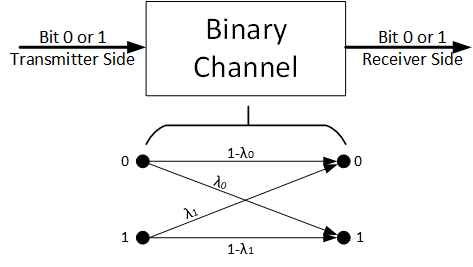
\includegraphics[scale=0.9]{Figures/BinaryChannel}
\caption{Binary Channel.}
\label{fig:binarychannel}
\end{figure}
\begin{eqnarray}
\nonumber
P_0~=~Bernoulli\left(\lambda_0\right),~i.e. P_0\{1\}&=&\lambda_0\\
\nonumber
P_0\{0\}&=&1-\lambda_0
\end{eqnarray}
\begin{eqnarray}
\nonumber
P_1~=~Bernoulli\left(1-\lambda_1\right),~i.e. P_1\{1\}&=&1-\lambda_1\\
\nonumber
P_1\{0\}&=&\lambda_1
\end{eqnarray}
\par The corresponding likelihood ratio is,
\begin{equation}
\nonumber
L(y) = \frac{p_1(y)}{p_0(y)} = 
\begin{cases}
	\frac{\lambda_1}{1-\lambda_0} ~~~~~~~\mbox{if}~ y=0, \\
	 \frac{1-\lambda_1}{\lambda_0} ~~~~~~~\mbox{if}~ y=1.
\end{cases}
\end{equation}
As we have already seen that Bayesian decision rule is liklihood ratio test, having following form,
\begin{equation}
\nonumber
\delta_B(y)=\mathbbm{1}~{\{L(y)\geq \tau\}},
\end{equation}
where $\tau= \frac{\pi_0(C_{10}-C_{00})}{\pi_1(C_{01}-C_{11})}$ is a threshold, which depends on the prior probabilities and the costs. For this case the Bayesian decision rule $\delta_{B}(y)$ is given as,
\begin{eqnarray}
\nonumber
\delta_{B}(0)=
\begin{cases}
1,~~~\mbox{if}~\lambda_1\geq\tau(1-\lambda_0),\\ 
0,~~~\mbox{if}~\lambda_1<\tau(1-\lambda_0).
\end{cases}\\ \nonumber
\delta_{B}(1)=\begin{cases}
1,~~~\mbox{if}~(1-\lambda_1)\geq\tau\lambda_0,\\
0,~~~\mbox{if}~(1-\lambda_1)<\tau\lambda_0.
\end{cases}
\end{eqnarray}
\par Let us consider the simple case of uniform cost, for which, $C_{ij} = 0~ \mbox{if}~ i=j$ and $C_{ij} = 1~ \mbox{if} ~i\neq j$, and equal prior probabilities i.e.,  $\pi_0=\pi_1=1/2$. In this case, $\tau=1$, and the Bayesian decision rule is given as,
\begin{eqnarray}
\nonumber
\delta_{B}(0)=
\begin{cases}
1,~~~\mbox{if}~\lambda_1\geq(1-\lambda_0),\\ 
0,~~~\mbox{if}~\lambda_1<(1-\lambda_0).
\end{cases}\\ \nonumber
\delta_{B}(1)=\begin{cases}
1,~~~\mbox{if}~(1-\lambda_1)\geq\lambda_0,\\
0,~~~\mbox{if}~(1-\lambda_1)<\lambda_0.
\end{cases}
\end{eqnarray}
Equivalently this can be written as,
\begin{equation}
\nonumber
\delta_{B}(y)=\begin{cases}
y,\hspace{35pt}\mbox{if}~\lambda_1+\lambda_0\leq1\\
\left( 1-y\right), ~\mbox{if}~\lambda_1+\lambda_0>1.
\end{cases}
\end{equation}
For Binary Symmetric Channel, where $\left(\lambda_1=\lambda_0=\lambda\right),\delta_B(y)$ can be written as,
\begin{equation}
\nonumber
\delta_{B}(y)=\begin{cases}
y,\hspace{35pt}\mbox{if}~\lambda\leq  0.5\\
\left( 1-y\right), ~\mbox{if}~\lambda>0.5.
\end{cases}
\end{equation}
\end{exmp}


\begin{exmp}[Location testing with Gaussian error]
The input to the channel is real numbers, here there are two possible inputs $\mu_0$ and $\mu_1$. The gaussian noise is added to the input and the output is produced. This is very commonly used model in many communication application and measurement application. The goal here is to guess which of $\mu_0$ or $\mu_1$ was sent.\\


\begin{figure}[h]
\centering
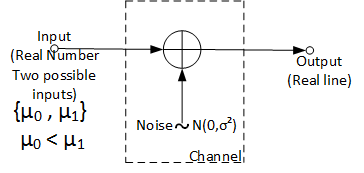
\includegraphics[scale=1]{Figures/LocationTesting}
\caption{Location Testing with Gaussian Error.}
\label{fig:LocationTest}
\end{figure}
\begin{align*}
\Gamma &\bydef \Re\\
H_j &= \mu_j \in \Re \text{ is the input, j = \{0,1\}}\\
\mathbbm{P}_j &= N(\mu_j,\sigma^2)\\
\end{align*}
{\Large
\begin{align*}
L(y)=\frac{p_1(y)}{p_0(y)}&=\frac{\frac{e^{\frac{-(y-\mu_1)^2}{{2\sigma}^2}}}{\sqrt{2\pi{\sigma}^2}}}{\frac{e^{\frac{-(y-\mu_0)^2}{{2\sigma}^2}}}{\sqrt{2\pi{\sigma}^2}}}\\
&=e^{\frac{-(y-\mu_1)^2+y-\mu_0)^2}{2{\sigma^2}}}\\
&=e^{\frac{(\mu_1-\mu_0)(2y-\mu_0-\mu_1)}{2{\sigma}^2}}\\
&=e^{\frac{(\mu_1-\mu_0)(y-\frac{\mu_0+\mu_1)}{2}}{{\sigma}^2}} (\geq \tau)\\
\end{align*}
}
\begin{align*}
\text{Therefore, A Bayes rule is of form }\\
\delta_B(y) &= \indic{L(y) \geq \tau}  \\
&=\indic{y \geq \frac {\mu_0+\mu_1}{2}+\frac{{\sigma}^2 \ln\tau}{\mu_1-\mu_0}}\\
\end{align*}


The RHS of the above inequality can be represented as some constant 
$\tau^1$.\\
$\tau^1$ 
 is determined without looking at output, Rather it is determined by simply looking at the model of the channel.\\
\begin{align*}
\delta_B&= \indic{y \geq \tau^1}\\
\end{align*}
\subsubsection{\em Special case}  Computing Bayes' decision rule under Uniform costs and Equal prior (Threshold based on average).For uniform cost, $\tau=1$, so $\ln\tau=0$.\\
Hence,
\begin{align}
\delta_B(y) = \indic{y \geq \frac{\mu_0+\mu_1}{2}}
\end{align}

\begin{figure}[h]
\centering
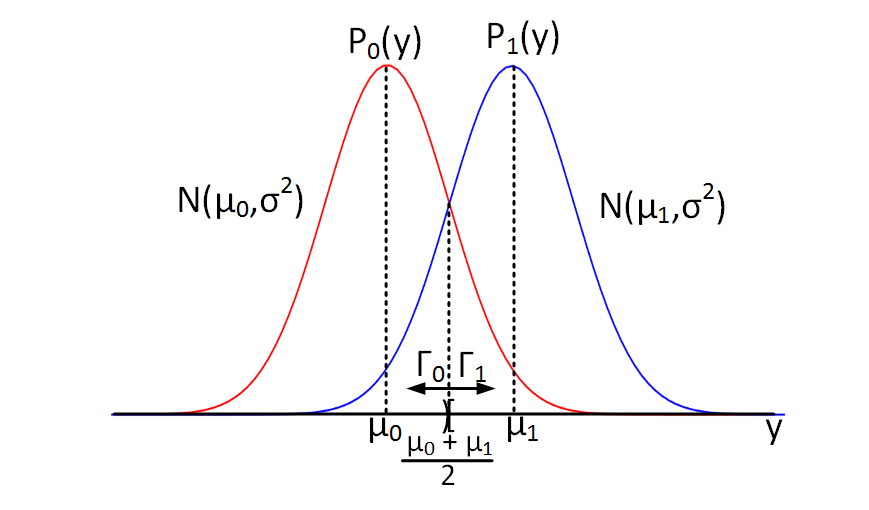
\includegraphics[scale=0.5]{Figures/Gaussian}
\caption{Illustration of location testing with Gaussian Error,unifrom costs, and equal priors}
\label{fig:Gaussian}
\end{figure}




Its Bayes risk is 
\begin{align*}
r(\delta_B)&= \pi_0 R_0+\pi_1 R_1 \\
&=\frac{(R_0+R_1)}{2}\\
\text{since uniform prior, }
R_0 = R_1\\
r(\delta_B) &= \int_{\frac{\mu_0+\mu_1}{2}}^{\infty}{\frac{1}{\sqrt(2 \pi {\sigma}^2)}}e^{-\frac{(z-\mu_0)^2}{2 {\sigma}^2}} dz\\
\text{Using the substitution    }
y&=\frac{z-\mu_0}{\sigma}\\
 &= \int_{\frac{\mu_1-\mu_0}{2}}^{\infty}{\frac{1}{\sqrt(2 \pi)}e^{-\frac{y^2}{2 }}} dy \\
&=1-\Phi{(\frac{\mu_1-\mu_0}{2\sigma})} 
\text{   Where $\Phi$ is Gaussian CDF}\\
\text{Define }
d &\bydef \frac{\mu_1-\mu_0}{\sigma}\\
\end{align*}
   Where "d" is defined as the Signal to Noise ratio of the system/channel \\
\begin{align}
r(\delta_B) = 1-\Phi{(\frac{d}{2})}
\end{align}

\begin{figure}[h]
\centering
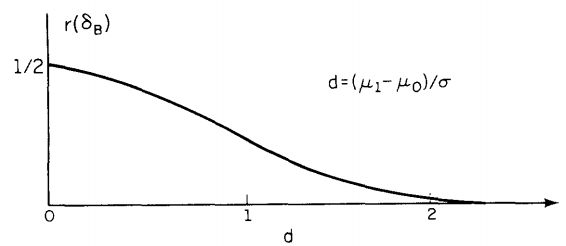
\includegraphics[scale=0.7]{Figures/BayesRisk}
\caption{Bayes Risk in location testing with Gaussian Error}
\label{fig:BayesRisk}
\end{figure}





\end{exmp}
















\end{itemize}
\end{document}





